\documentclass[main.tex]{subfiles}

\begin{document}

\chapter{Класична аналогија ЕИТ-а}%
\label{cha:klasik_eit}

\section{Увод}%
\label{sec:uvod}

У ласерској физици, електромагнетно-индукована транспаренција (ЕИТ) је позната као ефекат који поништава утицај средине на пропагирајући сноп~\cite{harris1990nonlinear}. Типично, ради се о систему са три нивоа (у тзв. $\Lambda$ конфигурацији, приказаној на сл.~\ref{fig:sl_eit/lambda}), где је прелаз између стања $\ket{1}$ и $\ket{3}$ забрањен за диполе (односно, стање $\ket{3}$ је метастабилно). Затим, два ласерска снопа, пумпајући и пробни, се спрежу са прелазима $\ket{1}\to\ket{3}$ и $\ket{1}\to\ket{2}$, респективно. Ако је остварена одговарајућа кохеренција, вероватноћа да се атом нађе у екситованом стању нестаје, због чега пробни сноп пропагира без апсорпције.

Могуће је успоставити аналогију између елемената матрице густине и спрегнутих класичних осцилатора – у оба случаја, динамика система је описана формално еквивалентним једначинама. Одговарајућа спрега између осцилатора може се јавити у различитим системима, као што су нпр. спрегнути механички/електрични осцилатори, при чему је ефекат познат под називом \emph{класична аналогија ЕИТ-а}. За остваривање, потребно је имати два или више резонатора, који су различито спрегнути са спољашњом побудом – слабо спрегнути, тзв. тамни елемент, са великим $Q$-фактором, и јако спрегнути, тзв. светли елемент, са ниским $Q$-фактором.

Од посебног интереса је реализација класичног ЕИТ-а у метаматеријалима који се састоје од спрегнутих резонатора. Ефекат се манифестује као оштар трансмисиони максимум у оквиру апсорпционе линије~\cite{tassin:09,cihan,mr05}. Пропраћен је наглашеном дисперзијом, која резултује високом вредношћу групног кашњења, односно малом групном брзином. Измерене су вредности више од 200 пута спорије пропагације таласа него у слободном простору, што чини ову врсту метаматеријала погодним за примене са успоравањем светлости у терахерцном опсегу~\cite{tassin:09}, као и за линије за кашњење у микроталасном опсегу~\cite{mr05}. Такође, због високог $Q$-фактора и израженог конфинирања поља, резонантни максимум је веома осетљив на промене индекса преламања у окружујућој средини, што је пожељно за сензорске примене.
\begin{figure}[h]
    \centering
    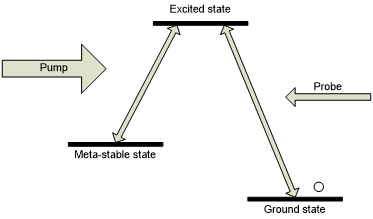
\includegraphics[width=0.8\linewidth]{sl_eit/lambda.png}
    \caption{sl_eit/Lambda}
    \label{fig:sl_eit/lambda}
\end{figure}
\begin{figure}[h]
    \centering
    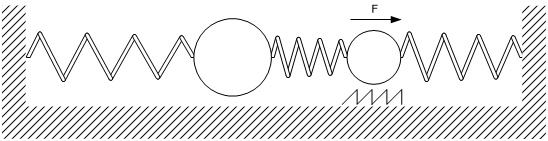
\includegraphics[width=0.8\linewidth]{sl_eit/opruge.png}
    \caption{sl_eit/Opruge}
    \label{fig:sl_eit/opruge}
\end{figure}

организација...

\section{Модел спрегнутих осцилатора}%
\label{sec:model_spregnutikh_ostsilatora}

На сл.~\ref{fig:sl_eit/opruge} је приказан систем два спрегнута механичка осцилатора, који ће бити коришћен за објашњење механизма класичне аналогије ЕИТ-а. Претпоставимо да честице обележене са 1 и 2 имају масе $m_1$ и $m_2$, респективно. Оба осцилатора, када нису спрегнута (тј. без опруге у средини), имају исту резонантну учестаност $\omega_0$, док је константа слабљења за честицу 2 много мања него за честицу 1, $\gamma_2\ll\gamma_1$. Коефицијент спреге је $\kappa$. Онда, ако спољашња синусоидална сила делује на честицу 1, $F=F_0e^{j\omega t}$, једначине кретања имају следећи облик ($x_{1,2}$ представља растојање одговарајућих честица од њиховог равнотежног положаја):
\begin{align}
    \label{eq:spreg_osc}
    \frac{\partial^2x_1}{\partial t^2} + \gamma_1 \frac{\partial x_1}{\partial t} + \omega_0^2 x_1 + \kappa x_2 & = F = F_0 e^{j\omega t}, \label{eit:jkr1} \\
    \frac{\partial^2 x_2}{\partial t^2} + \gamma_2 \frac{\partial x_2}{\partial t} + \omega_0^2 x_2 + \kappa x_1 & = 0.\label{eit:jkr2}
\end{align}
У овој аналогији, сила $F$ представља упадни талас чија трансмисија се мери (пробни талас), ... ПРОВЕРИ АНАЛОГИЈУ (ПОШТО ОВО КАКО ЈЕ НАВЕДЕНО НИЈЕ ТАЧНО)!!

Кретање честице 1 је повезано са апсорпцијом због трења; уколико ова честица мирује, апсорпција неће бити присутна. Решавањем система (\ref{eit:jkr1})–(\ref{eit:jkr2}) добија се следећи израз за померај:
\begin{equation}
    \label{eq:pomeraj}
    x_1 = \frac{\left( \omega_0^2 - \omega^2 + j\omega\gamma_2 \right)F_0}{\kappa^2 + \left( \omega_0^2 - \omega^2 + j\omega\gamma_1 \right) \left( \omega_0^2 - \omega^2 + j\omega\gamma_2   \right)}.
\end{equation}
Из (\ref{eq:pomeraj}) се види да је померај прве честице, на резонантној учестаности $\omega_0$, пропорционалан константи слабљења друге честице, $\gamma_2$, за који је претпоставка да је веома мали, због чега је и апсорпција такође мала. У граничном случају $\gamma_2\to 0$, очигледно је да $x_1$ такође тежи нули, дакле апсорпција у систему је у потпуности уклоњена.

\section{Преглед литературе}%
\label{sec:pregled_literature}

Један од првих покушаја да се испита аналогија између ЕИТ-а и спрегнутих резонатора у метаматеријалима дата је у реф.~\cite{tassin:09}. Коришћени су сплит рингови са асиметричним процепима, или асиметрично постављени у односу на спољашње поље, како би се обезбедила асиметрична побуда. Такође су коришћени диелектрици са различитим тангенсом губитака, како би се остварила потребна разлика у факторима доброте. Остварена је вредност групног индекса око 100, уз истовремено веома мале губитке у трансмисији. Други рад истих аутора користи другачији приступ, са различитим врстама резонатора (сплит ринг и кратке жице), како би се остварила разлика у $Q$-факторима~\cite{tassin2009planar}. Како би се избегла ограничења због губитака у металима, предложено је коришћење суперпроводних ниобијумских (Nb) филмова~\cite{cihan}. Додатна предност овог приступа је могућност укључивања/искључивања ефекта регулацијом температуре.

\bibliographystyle{babplai3}
\bibliography{ref}

\end{document}
